\documentclass[12pt,twoside,letterpaper]{article}
\setlength\topmargin{0in}
\setlength\headheight{0in}
\setlength\headsep{0in}
\setlength\textheight{9.0in}
\setlength\textwidth{6.5in}
\setlength\oddsidemargin{0in}
\setlength\evensidemargin{0in}
\setlength{\parskip}{12pt}
\pagestyle{empty}
\raggedright
\usepackage{graphicx}
\title{Developing Scale in Eclipse}
\author{Cameron Palmer}
\date{November 2008}
\begin{document}
\maketitle
The most recent version of Scale is completely Java-based, which means you should be able to develop for the Scale compiler in Eclipse on just about any OS and hardware. The original frontend was limited because it relied on the EDG library that would only run in certain environments. Today that code has been replaced by the Java-based ANTLR.

\section*{Requirements}
\begin{itemize}
\item Eclipse 3.4.1 (Ganymede)
\item Java JDK 1.5 or later
\item GNU make
\end{itemize}

\section*{Downloading Scale}
The official Scale website is http://www-ali.cs.umass.edu/Scale/. The Scale project is migrating from UMass to University of Texas at Austin so this site may move.

First we need to checkout the scale source using the subversion (http://subversion.tigris.org/) version control utility.
\begin{verbatim}
svn co  http://z.cs.utexas.edu/svn/scale/trunk my-scale
\end{verbatim}

\section*{Creating the necessary environment}
In the my-scale directory you can create an env.sh file that contains the following. May need to be edited for your environment.

\begin{verbatim}
echo "setting up environment at base $PWD"

SCALE="$PWD"; export SCALE
SCALEHOME="$SCALE/scale"; export SCALEHOME
SCALEDOC="$SCALE/doc"; export SCALEDOC

SCALEHOST="$(uname)"; export SCALEHOST
SCALEHOSTNAME=""; export SCALEHOSTNAME
SCALEHOSTTYPE="i386"; export SCALEHOSTTYPE
SCALERELEASE=""; export SCALERELEASE
SCALETARGETTYPE="sparc"; export SCALETARGETTYPE

CLASSDEST="$SCALEHOME/classes"; export CLASSDEST
CLASSPATH="$CLASSPATH:$SCALE:$SCALEHOME/classes:$SCALEHOME/frontend/antlr.jar"
export CLASSPATH
JAVA="java"; export JAVA
JAVAC="javac"; export JAVAC
JAVACFLAGS="-J-Xmx256m -d $CLASSDEST -g"; export JAVACFLAGS

JAVAD="javadoc"; export JAVAD
JAVADDEST="$SCALEDIR/doc/html"; export JAVADDEST
JAVADFLAGS="-J-Xmx128m -J-Xms32m"; export JAVADFLAGS
JAVAH="javah"; export JAVAH
\end{verbatim}

After creating the env.sh file you need to source it. Then change to my-scale/scale/. Create the classes folder where your class files will end up after compilation.
\begin{verbatim}
$ . ./env.sh
$ cd scale
$ mkdir classes
\end{verbatim}

Next you need to compile the ANTLR grammars in my-scale/scale/frontend. This will cause ANTLR to generate the necessary frontend lexer and parser code from the C and Fortran grammars.
\begin{verbatim}
$ cd frontend
$ make
\end{verbatim}

\section*{Creating the project in Eclipse}
Create a new Java project in Eclipse by clicking File $\rightarrow$ New $\rightarrow$ Java Project. Give the project an appropriate name, create project from existing source and then click Next as in Figure \ref{fig:create_java_project}.
\begin{figure}[htp]
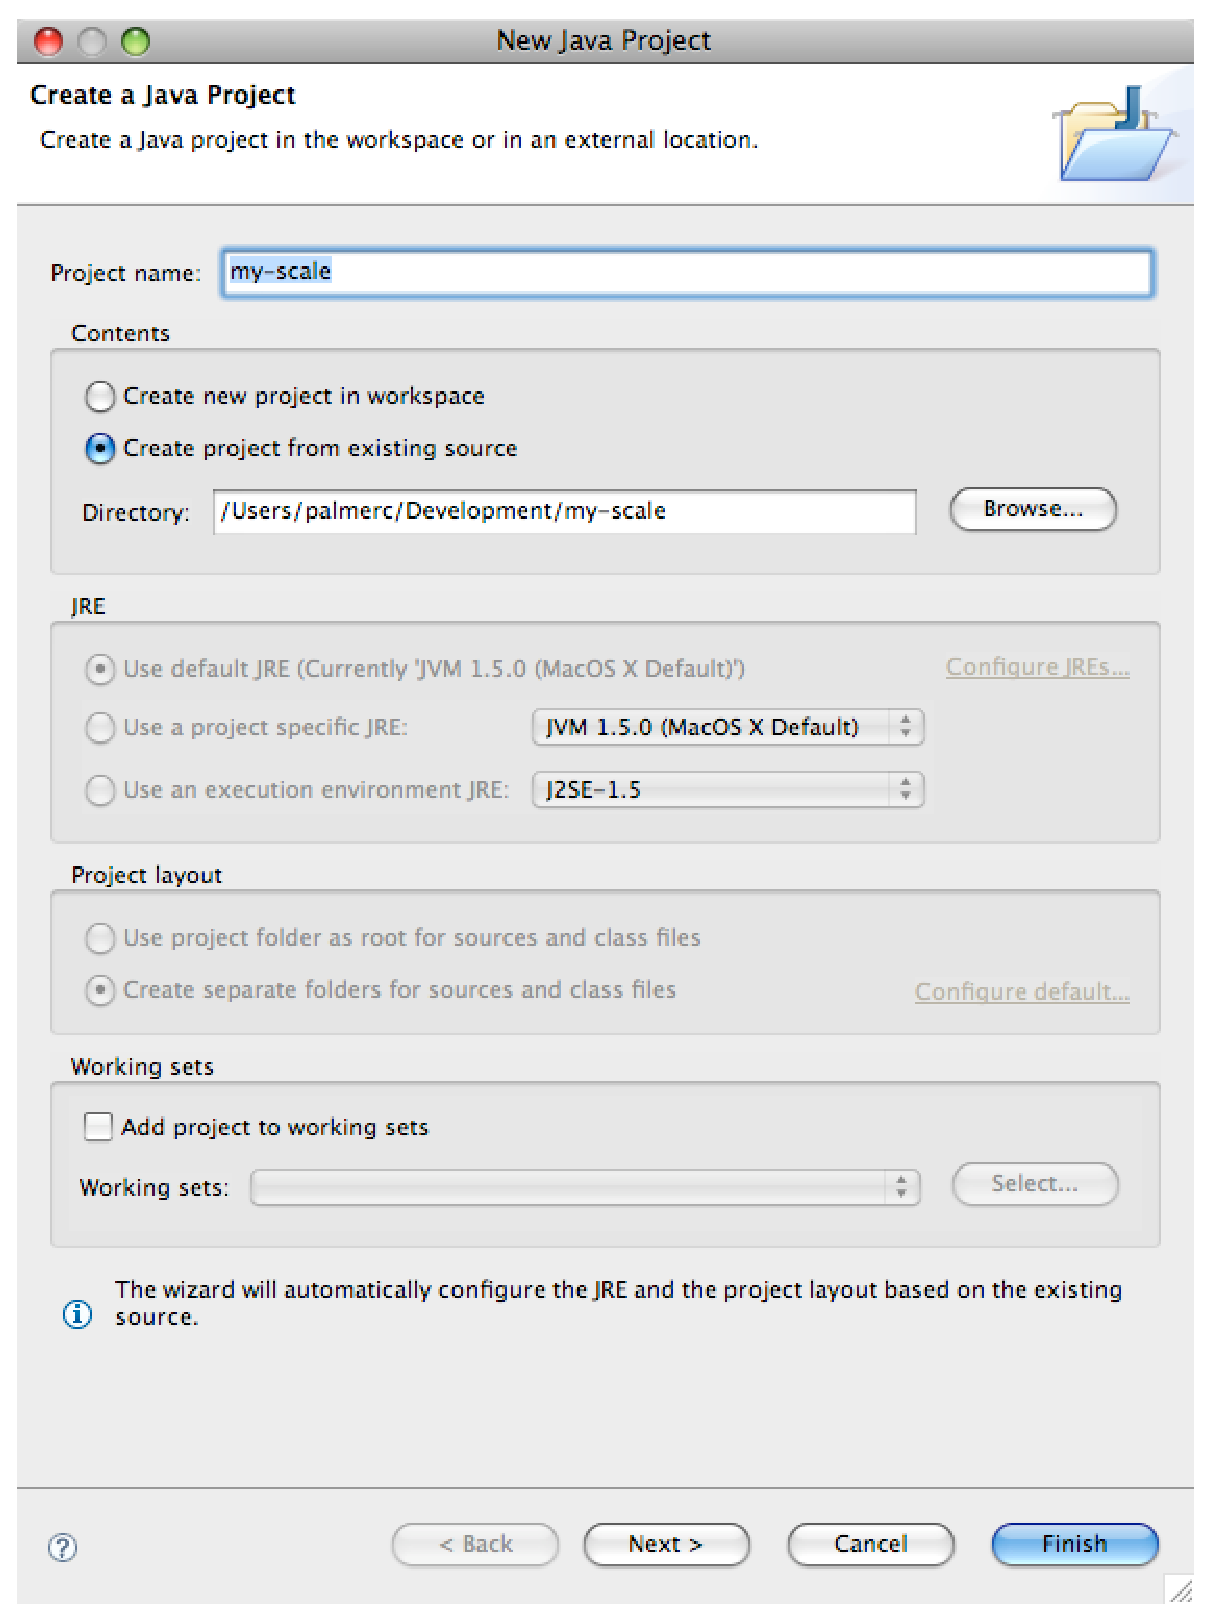
\includegraphics[width=150mm]{create_java_project.eps}
\caption{Creating a new Java project for Scale}\label{fig:create_java_project}
\end{figure}

Check the Source tab to make sure Default output folder is set correctly. We use my-scale/scale/classes in Figure \ref{fig:create_java_project_source}.
\begin{figure}[htp]
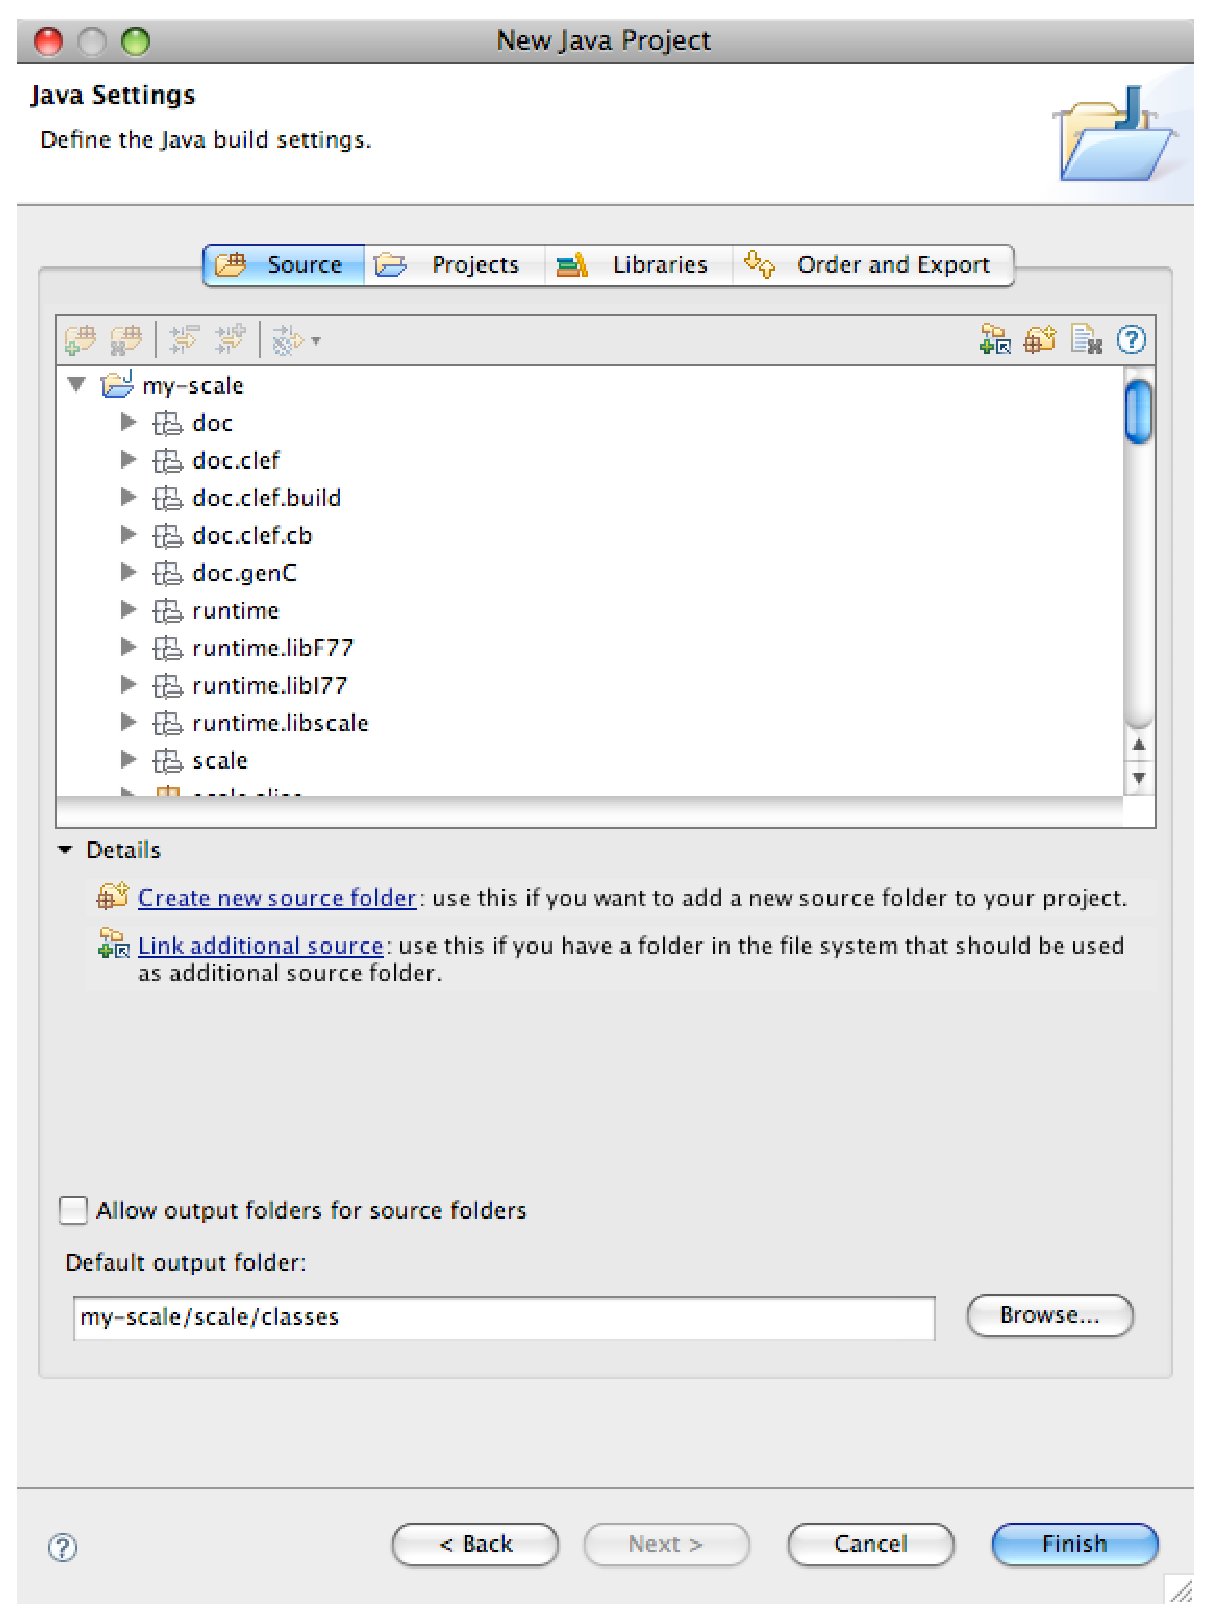
\includegraphics[width=150mm]{create_java_project_source.eps}
\caption{Set the classes ouput folder for the project}\label{fig:create_java_project_source}
\end{figure}

Finally, under libraries add a JAR. Point to the my-scale/scale/frontend/antlr.jar as in Figure \ref{fig:create_java_project_libraries}. After this you should be ready to develop with Scale and Eclipse.
\begin{figure}[htp]
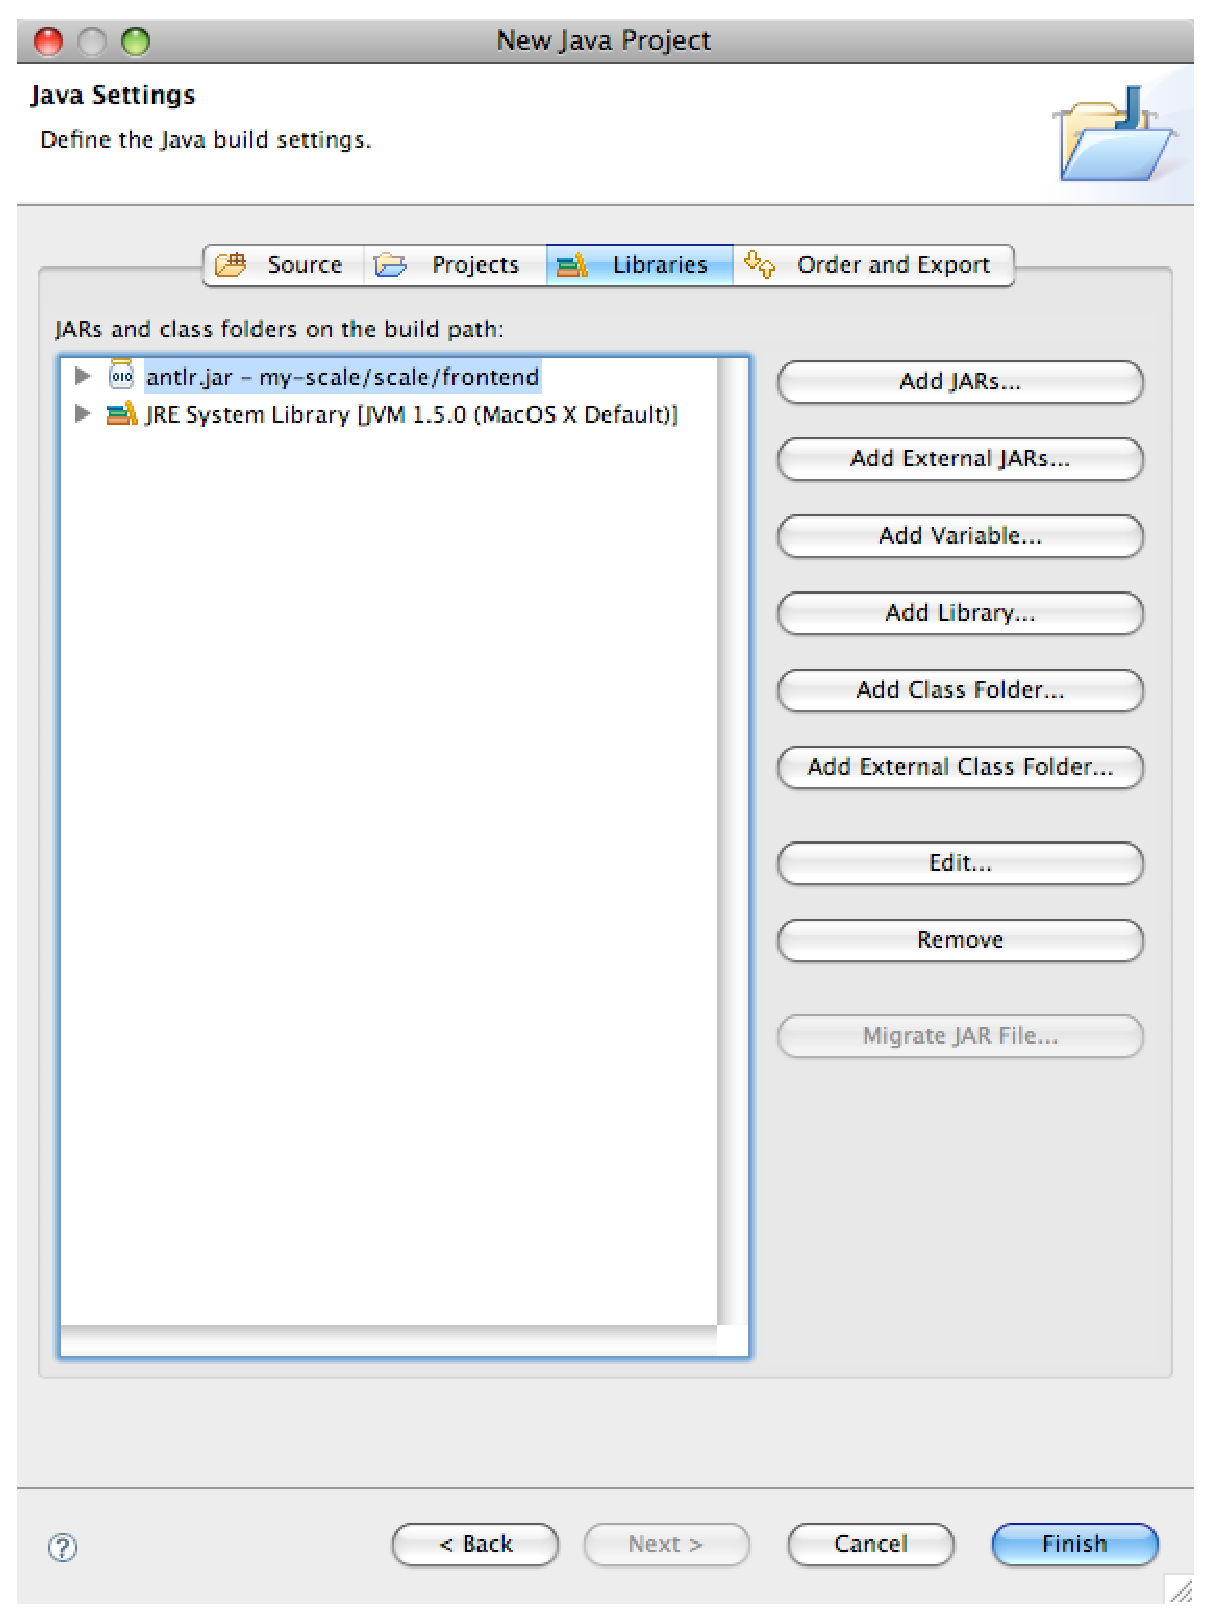
\includegraphics[width=150mm]{create_java_project_libraries.eps}
\caption{Make sure antlr.jar is in the classpath}\label{fig:create_java_project_libraries}
\end{figure}

\section*{Create a run configuration}
Click Run $\rightarrow$ Run Configurations. Double-click Java Application to create a new configuration. As in Figure \ref{fig:run_java_application}, in the Main tab give the configuration a name and search for the correct Main class which is Scale - scale.test and click OK.
\begin{figure}[htp]
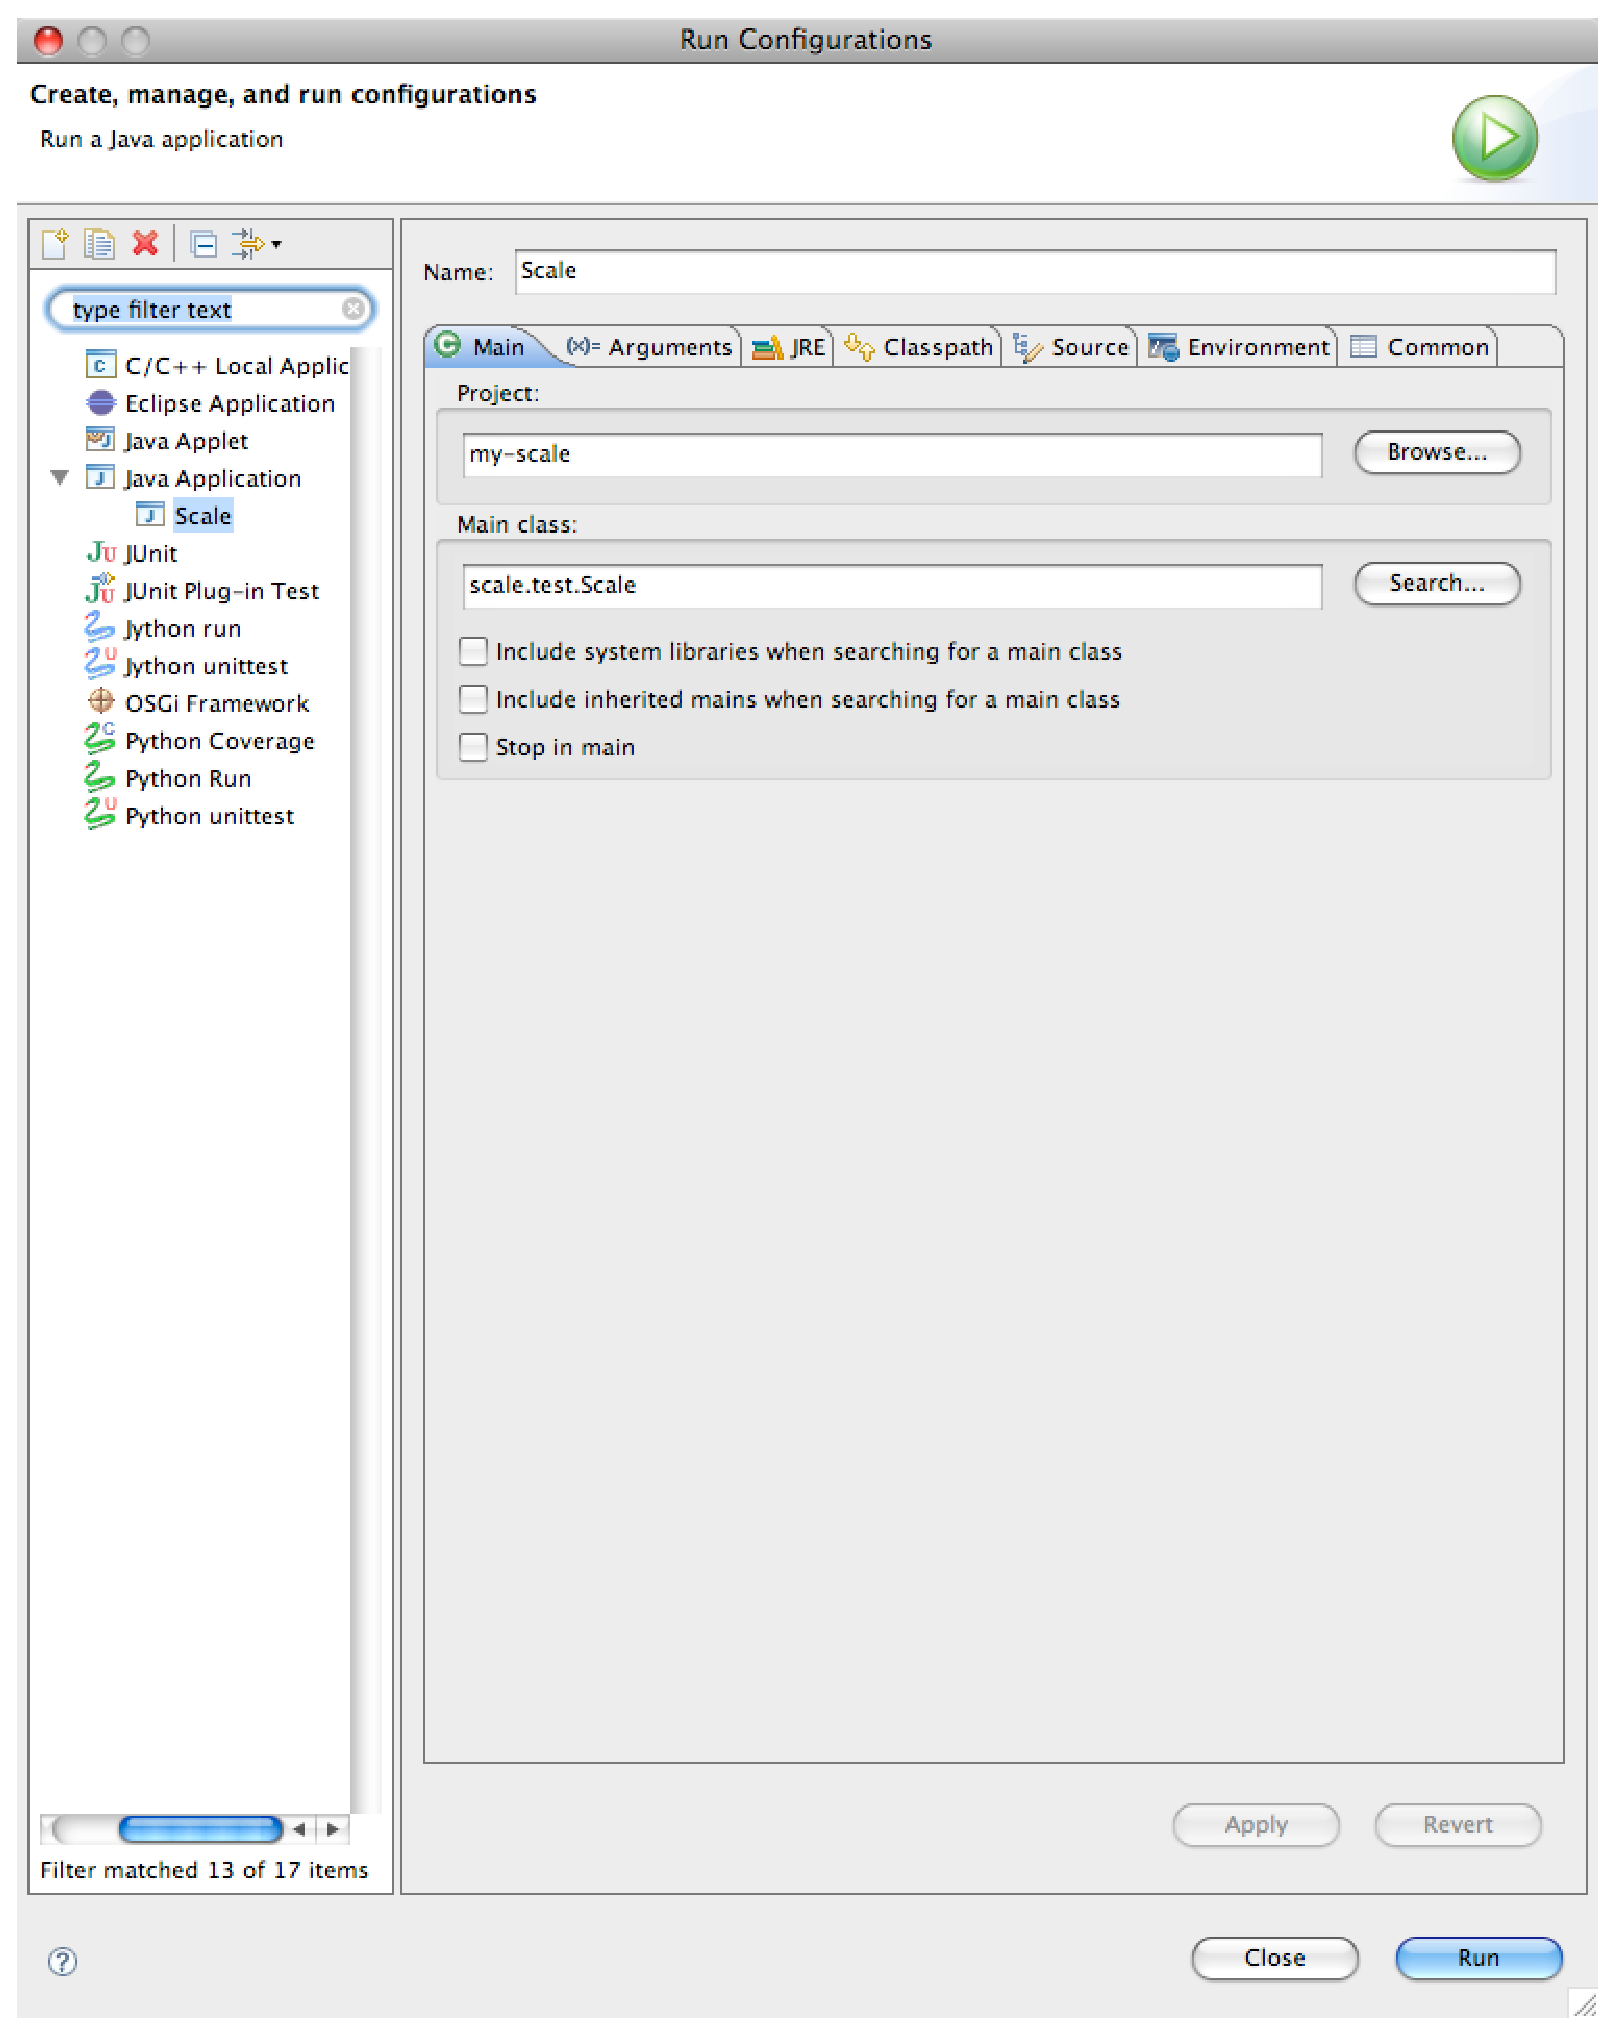
\includegraphics[width=150mm]{run_java_application.eps}
\caption{Setting up main part of the Run Configuration}\label{fig:run_java_application}
\end{figure}

On the Arguments tab give the appropriate Program arguments as in Figure \ref{fig:run_java_application_arguments}. For starters you could add -help. This would cause the help page to display everytime the application runs. A more useful option would be -arch sparc -oa hello.c. This would generate a sparc assembly file of whatever was contained in hello.c. You can do the same thing at the command-line.
\begin{verbatim}
$ cd my-scale
$ . ./env.sh
$ java scale.test.Scale -arch sparc -oa hello.c
\end{verbatim}
\begin{figure}[htp]
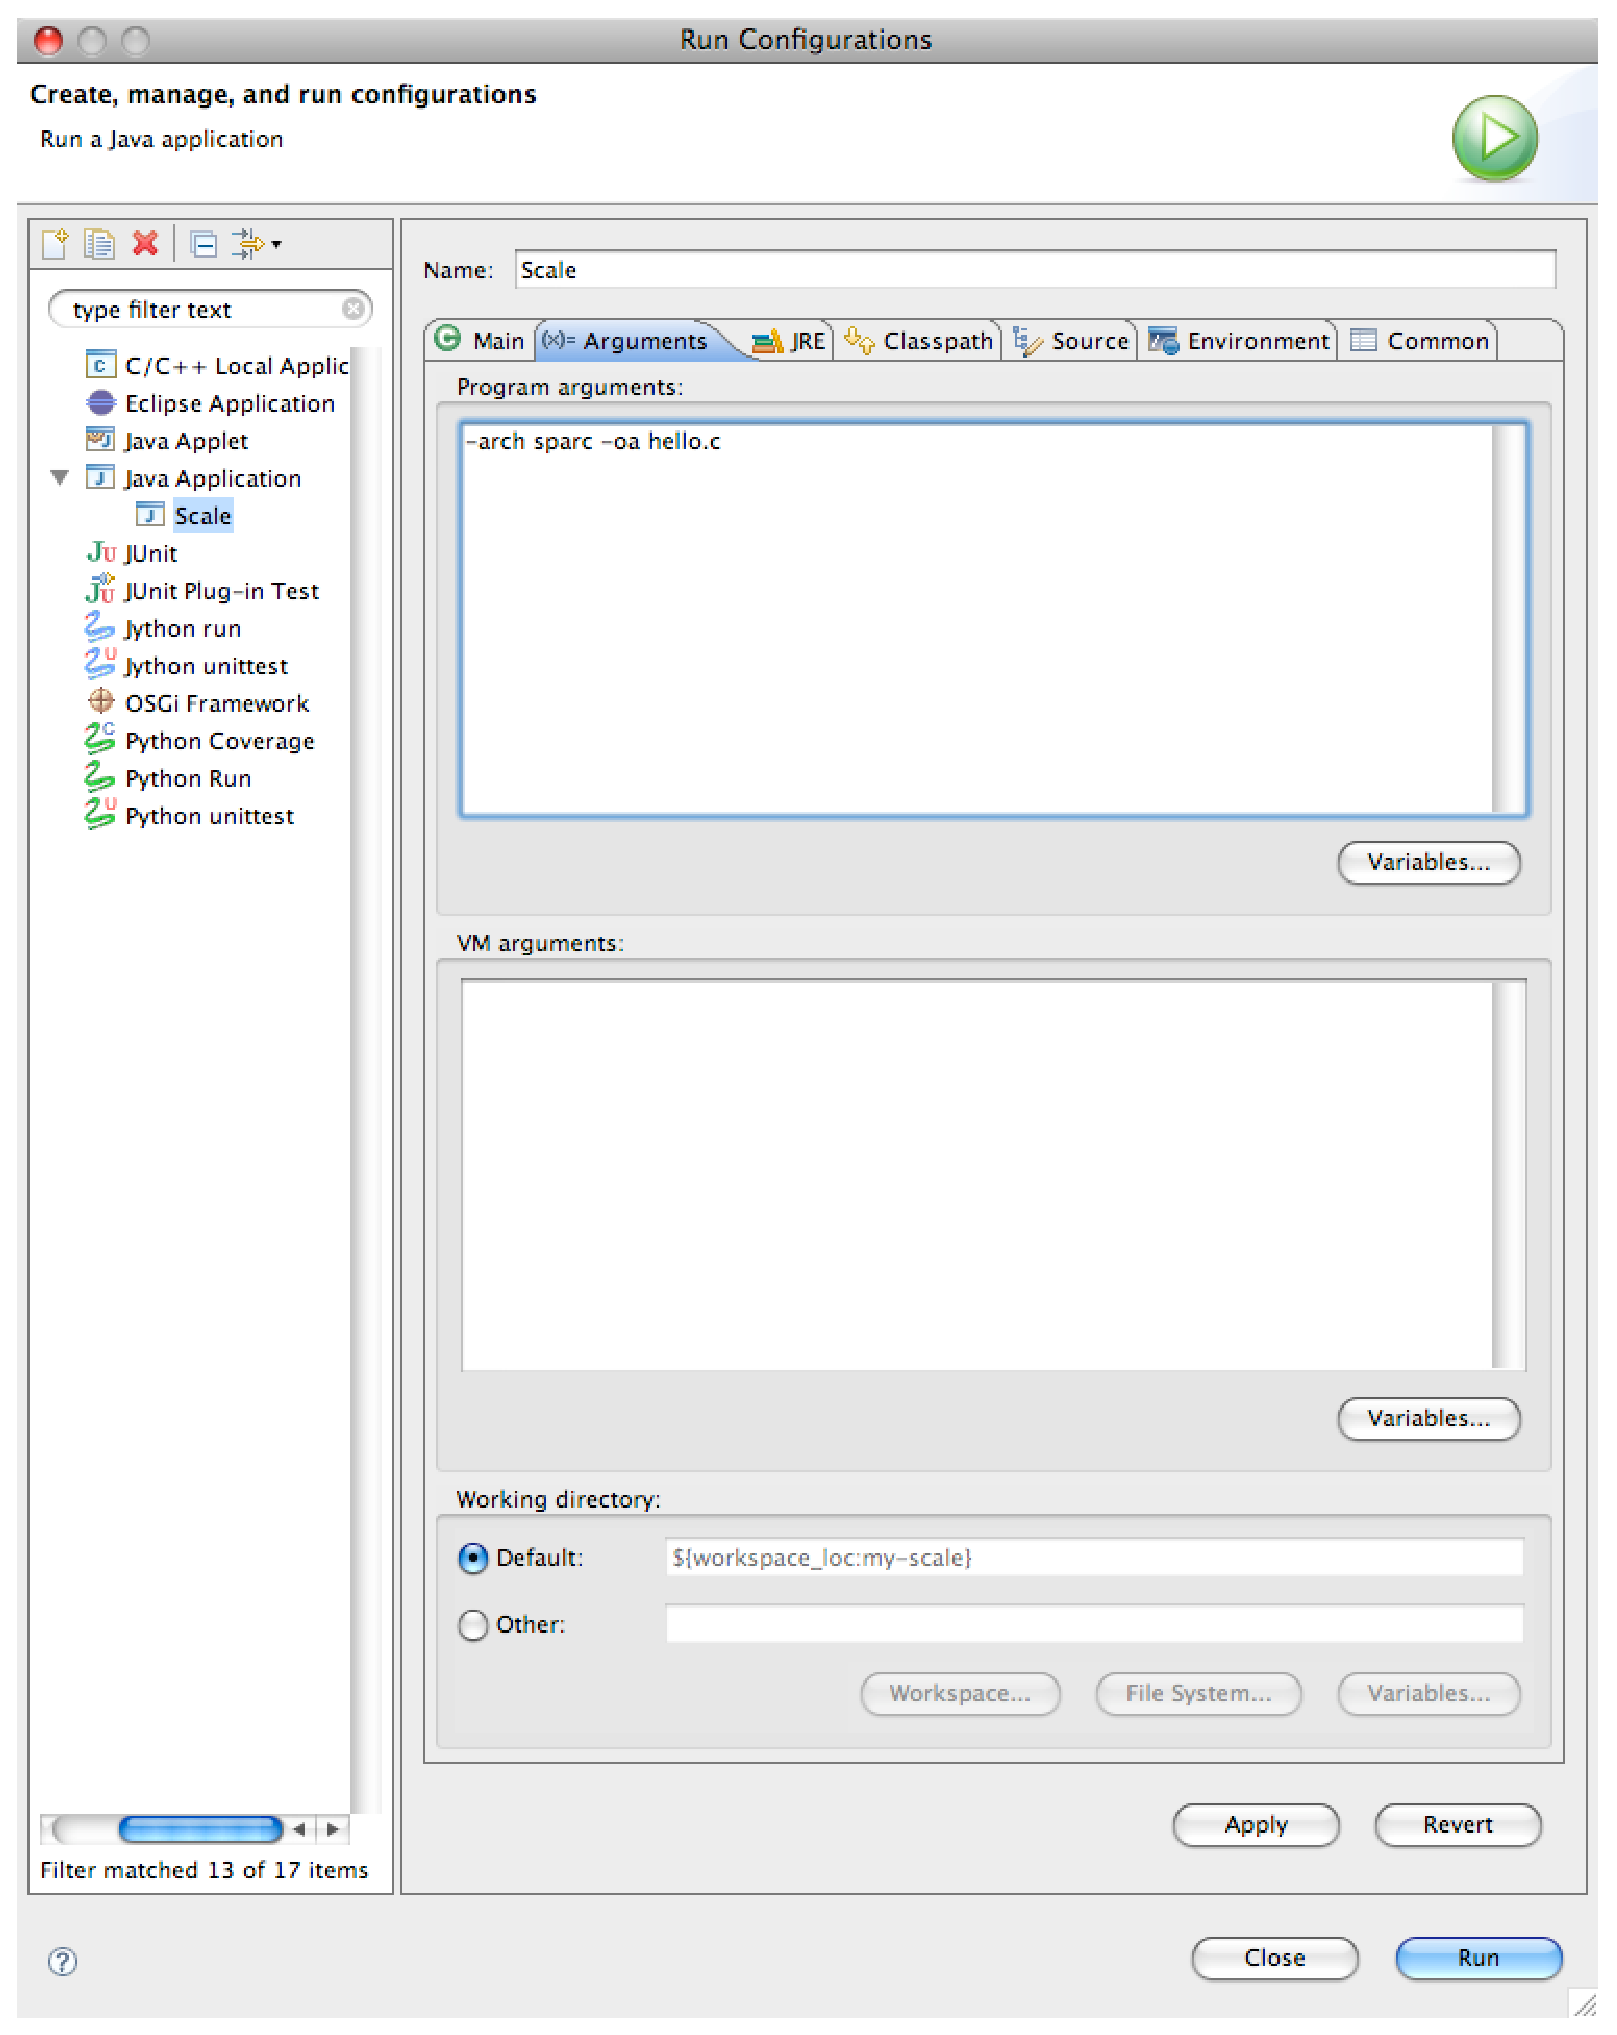
\includegraphics[width=150mm]{run_java_application_arguments.eps}
\caption{The arguments for the application}\label{fig:run_java_application_arguments}
\end{figure}

\end{document}